\section{Introduction To One Dimensional Dynamics}

\begin{defn}[Fixed Point]
	Assuming we have a iterated dynamical system $x_{i+1} = f(x_i)$. 
	The fix point of $f$ is a point $x^*$ such that $f(x^*) = x^*$. 
	That is, the fixed points are the solution to the equation $f(x) = x$.
\end{defn}

Fixed points are like sinks in the dynamical system. 
If for some $c$ there exists a $n$ such that $f^n(c) = x^*$, $c$ will stay at $x^*$ forever. 
Our intuition tells us that the fixed points shall determine, at least in parts, the properties of the dynamical system.
In deed, for some dynamical system $f = x$ for all $x \in I$, where $I$ is some interval, what takes place in that interval would not be so interesting.

Many interesting dynamical system have infinitely many fixed point, but the set of fixe point is of measure zero, meaning if picking any point in the interval at random, there is a zero chance that it is a fixed point.
Two traditional examples for a set of measure zero are rational points and cantor set on the real axis. 

Given a fixed point, it is natural to ask what are the behaviors of the dynamical system nearby it.
Will nearby points converge to it, or diverge from it?
It turns out both are simplifications, and the proper description of the behavior is that it will either be a \emph{stable} fixed point or an \emph{unstable} one. 

Here is the rigorous definition of stability, attributed to the renowned Russian mathematician Aleksandr Mikhailovich Lyapunov \cite{lyapunov}.

\begin{defn}[Stable fixed point]
A fixed point $x^*$ is stable if for all $\epsilon$ there exists a $\delta$ such that 
$$
	|f^n(x) - f^n(x^*)| < \epsilon \text{ for } n = 1,2, \cdots 
$$
whenever $|x - x^*| < \delta$.
Here $f^n$ denotes the composition of $f$ $n$ times.
\end{defn}

The intuition for the definition is that if $x$ is close enough to a stable fixed point $x^*$, it will stay close to it forever. 
It does not imply, however, all $x$ close to $x^*$ will converge to it.
The classical example for 1-dimension case is the identity map $f(x) = x$. 
All points are stable fixed points, but no points in a neighbourhood of the fixed point converges to it, except itself.

Considering the above example, we can define a stronger sense of stability called asymptotic stability.

\begin{defn}[Asymptotic Stability]
	A fixed point $x^*$ is asymptotically stable if it is stable and there exists a $\delta$ such that 
	$$
		\lim_{n \rightarrow \infty} f^n(x) = x^* \text{ whenever } |x - x^*| < \delta
	$$
\end{defn}

Upon settlement of this definition, the following theorem is immediate.

\begin{thm}[Stable and unstable fixed point]\label{th:_stable_unstable_fixed_point}
	If $x^*$ is a fixed point of a two time differentiable function $f$ and $|f'(x^*)| < 1$, $x^*$ is a  asymptotic stable fixed point.
	If $|f'(x^*)| > 1$, $x^*$ is unstable.
	If $|f'(x^*)| = 0$, $x^*$ may be stable or unstable.
\end{thm}

\begin{figure}
	\centering
	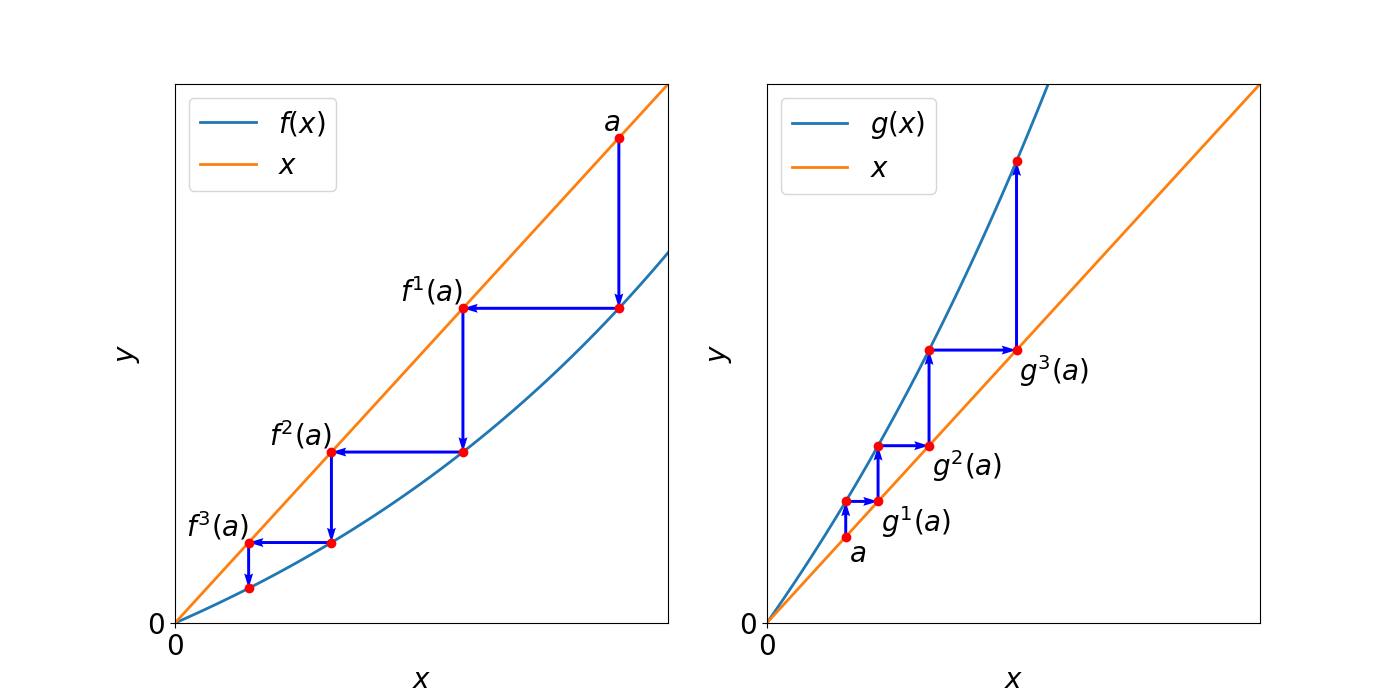
\includegraphics[width=\textwidth]{./figures/stable_and_unstable_fixed_point.png}
	\caption{An illustration of theorem \ref{th:_stable_unstable_fixed_point}.
	The figure on the left shows function $f(x) = 0.4 e^x - 0.4$, which has a stable fixed point at $x^* = 0$. 
	The figure on the right shows function $f(x) = 1.3 e^x - 1.3$, which has an unstable fixed point at $x^* = 0$.}
	\label{fig:stable and unstable fixed point}
\end{figure}

Figure \ref{fig:stable and unstable fixed point} is an illustration of this theorem.
To prove this theorem is a regular exercise using Taylor expansion. 

Assuming $x^*$ is a fixed point of the iterated map $f$ whose Taylor expansion is

$$f = f(x^*) + f'(x^*) (x - x^*) + O(x^2)$$

For any $\delta$ let is evaluate $f(x^* + \delta)$.
Since $x^*$ is a fixed point,
 $f(x^*) = x^*$, and
 $f(x^* + \delta) - f(x^*) = f'(x^*) \delta + O(x^2)$. 
For small enough $\delta$ we can ignore all the terms of degree higher than $2$, and the above equation states $x^*+ \delta$ will eventually converge to $x^*$ if $|f'(x^*)| < 1$, and diverge if $|f'(x^*)| > 1$.

This theorem, though simple, is powerful and is a fundamental part for any rigorous approach of iterated dynamical systems. 
As a result, hereby we give another proof using only the classic mean value theorem and $\epsilon-\delta$ definition of limit.

\begin{proof}[Proof of Theorem \ref{th:_stable_unstable_fixed_point}]
	Without loss of any generality we can assume that the stable fixed point is $0$, meaning $f(0) = 0$. 
	If the function $f^*$ has stable point not at $0$ but at $x^*$, we can always investigate the function $f(x) = f^*(x+x^*) - x^*$. 
	
	If for a neighbourhood of $0$ $f' = 0$, we are done, as by mean value theorem $f = 0$ in this neighbourhood, and every $x$ in this neighbourhood converges to $0$ after one iteration.

	If $f' \neq 0$, since $f'$ is continuous, there exists an interval around $0$ such that $f'(x)$ is either strictly positive or strictly negative in this interval (depending on the sign of $f'(x)$), and, since $|f'(0)| < 1$, we can further restrict the interval such that $|f'(x)| < c < 1$. 
	Label this interval as $I$. 
	Notice by construction, this interval is a neighbourhood of $0$, so it must contain $0$.
	
	First, consider $0 < f'(x) < 1$ for $x \in I$. 
	For any point $a<0$ and $a\in I$,  $f(a)$ must be small than $0$. 
	Otherwise, the function $f$ must be overall decreasing in the interval $(a, 0)$, which is impossible as in the whole interval $f'(x) > 0$. 
	Now, again, since $f'> 0$, $f(a) > a$, so the sequence $a, f(a), f^2(a), \cdots$ is monotonically increasing and bounded above by $0$. 
	By the completeness of the real number it must converge to some number. 
	Assuming it converges to $l < 0$. 
	Let us pick a point $a$ in the interval $(\frac{l}{c}, l)$. 
	That is, $a > \frac{l}{c} \implies \frac{l}{a} > c$ and $f(a) < l$.
	Notice 
	$$
	\frac{f(0) - f(a)}{0 - a} = \frac{f(a)}{a} > \frac{l}{a} > c
	$$
	Where $c$ is the constant defined above such that in the whole interval $|f'(x)| < c$.
	By mean value theorem, there exists a point $b$ in the interval $(a, 0)$ such that $f'(b) = \frac{f(a)}{a} > c$, which is a contradiction.

	All of other cases ( $a > 0, f'(0) < 1$) can be proved similarly.
\end{proof}

In the end, let us have some examples where the absolute value of the derivative at the fixed point is $1$.
Considering the function $f(x) = e^x - 1$, which has a fixed point at $0$.
All x smaller than $0$ will converge to $0$, while all $x$ larger than $0$ will diverge to infinity.

% TODO: more examples

\section{Devaney's Definition}

\begin{defn}[Topologically Transitive]
	Let $J$ be a set with a topology.
	The function $f: J \rightarrow J$ is topologically transitive, if for all non-empty open sets $U_1, U_2 \in J$, there exist $k \in \bb{N}$ such that $f^k(U_1) \cap U_2 \neq \varnothing$. 
	Here $f^k$ denotes the composition $\underbrace{f \circ f \cdots \circ f}_{k \text{ times}}$
\end{defn}

\begin{defn}[Dense]
	Let $X$ be subset of the topological space $J$. 
	$X$ is dense if $\overline{X} = J$, where $\overline{X}$ denote the closure of $X$.
\end{defn}

\begin{defn}[Periodic Point]
	A point $x$ is a period of period $k$ if $f^k(x)=x$.
\end{defn}

\begin{defn}[Sensitive Dependence on Initial Condition]
	This term is coined by Ruelle \cite{Ruelle-1978}.

	Let $J$ be a metric space with the metric $d: J \times J \rightarrow \bb{R}$.
	$f: J \rightarrow J$ has sensitive dependence on initial condition if there exists some $\delta > 0$ such that for all $x \in J$ and any neighbourhood $X$ containing $x$, there exists $y \in X$ and $n \in \bb{N}$ such that $d(f^n(x), f^n(y)) > \delta$.
\end{defn}

\begin{defn}[Chaos, Devaney's Definition]\label{def:Devaney_definition_for_chaos}
	Let $V$ be a metric space.
	A function $f: V \rightarrow V$ is chaotic if 
	\begin{enumerate}
		\item the set of periodic points are dense in $V$,
		\item $f$ is topologically transitive,
		\item $f$ has sensitive dependence on initial condition. 
	\end{enumerate}
	
\end{defn}


The definition here is attributed to Devaney \cite{Devaney_green_book_chaos_definition}. 
The first two requirements are purely topological, while the last one requires a metric. 
While in most circumstances topological properties are more generalised than the metric properties, here, surprisingly, as long as $V$ is a metric space (which is part of the assumption), the first two implies the third\cite{Banks}. 
As a result, we only need to check the first two conditions to determine if a function is chaotic.

\begin{thm}[Criterion For Chaotic Function]
	Let $V$ be a metric space. 
	Function $f: V \rightarrow V$ is chaotic as defined in \ref{def:Devaney_definition_for_chaos}
	if and only if its the periodic points are dense $V$ and it is topologically transitive,
\end{thm}

% TODO: Say more about doubling map. 
% TODO: graph, say more in introduction, etc?
% The doubling map is topologically transitive to the map in $S^1$

\begin{example}\label{ex_doubling_map}
	Recall the doubling map $f: [0,1) \rightarrow [0,1)$
	\begin{equation}\label{eq:doubling_map}
	f(x) = 
		\begin{cases}
			2x &\text{ if } 2x < 1 \\
			2x -1 &\text{ if } 2x > 1
		\end{cases}
	\end{equation}
	% TODO: more explanation
	This map can also be regarded as doubling the angles on the unit cycle: $g: S^1 \rightarrow S^1$ given by $ g(\theta) = 2 \theta$.
	
	The doubling map is \textit{chaotic}.

	All non-zero rational points $\frac{p}{q} \in [0,1)$ with odd denominater are periodic points for $f$. 
	The set of these points are dense.
	To show the periodicity, note the images of $\frac{p}{q}$ under repetitive applications of $f$ are $\frac{p}{q}, \frac{2p}{q}, \cdots, \frac{2^k p}{q}, \cdots$.
	We can regard all the numerators as the equivalence classes module $q$.
	Since this sequence is infinite and there are only finitely many possibilities for the numerators, some of the numerators must coincide. Let them be $2^k p$ and $2^{k'} p$. 
	Without loss of generacity let $k > k'$, and
	$$
	2^k p \equiv 2^{k'} p \mod q \implies 
	2^{k-k'} p \equiv p \mod q \text{ (as $q$ is odd)},
	$$
	which measn $f^{k-k'}(\frac{p}{q}) = \frac{p}{q}$, i.e., $\frac{p}{q}$ is a point of period $k - k'$.

	To show $f$ is topologically transitive is even easier. 
	For any non-empty open set $U \in [0,1)$, by definition there exists an open interval $J = (x, x+ \delta) \subseteq U$. 
	$J$ has diameter $\delta$, $f(J)$ has diameter $2 \delta$, and $f^k(J)$, $2^k \delta$. 
	Since the length of $[0,1)$ is $1$, after some finite iteration $f^k(J)$ would covers all of $[0,1)$ and intersect any other open sets.

	By generalising this proof it is clear any maps in the form 
	$$
	g: S^1 \rightarrow S^1; g(\theta) = r \theta, r \in R
	$$
	are chaotic.
\end{example}

To prove the doubling map is chaotic is a gentle exercise. 
To directly find the points of periodicity and prove that a general function is topologically transitive is difficult.
Instead, we can circumvent these challenges by exploiting certain topological properties introduced in the next section.

\section{Topological Conjugacy}

\begin{defn}[Topological Conjugacy]
Funcitons $f: X \rightarrow X$, $g:  Y \rightarrow Y$ are topologically conjugate if there exist a homeomorphism $\phi: X \rightarrow Y$ such that 
$\phi \circ f = g \circ \phi$,
i.e, the following diagram commutes.
\begin{center}
    \begin{tikzcd}
        X \arrow[r, "f"] \arrow[d, "\phi" swap] & X \arrow[d, "\phi"] \\
        Y \arrow[r, "g"] & Y
    \end{tikzcd}
\end{center}

The maps $f,g$ are semiconjugate if there exists a continuous surjection, $\psi$ such that $\psi \circ f = g \circ \psi$.
\end{defn}

% TODO: Shall we introduce a notation for topological conjugacy? 
% no notation is provided by Devaney or Wikipedia

To rephrase a definition, $f,g$ are conjugate if there exists and homeomorphism $\phi$ such that $f = \phi^{-1} \circ g \circ \phi$.
So $f^{n} = \phi^{-1} \circ g^{n} \circ \phi$; that is $f^n$ is conjugate to $g^n$.

Topological conjugacy is an equivalence condition. 
$f$ is conjugate to itself by identity map. 
$\phi \circ f = g \circ \phi$ implies $f \circ \phi^{-1} = \phi^{-1} \circ g$, so $g$ is also conjugate to $f$.
Lastly, if $f$  is conjugate to $g$ via $\phi$, and $g$ is conjugate to $h$ via $\phi'$, $\phi' \circ \phi \circ f = \phi' g \circ \phi = h \circ \phi'' $, which means $f$ is conjugate to $h$ via $h' \circ h$.

Topological semiconjugacy only requires a continuous surjection, $\psi$, such that $\psi \circ f = g \circ \psi$. 
As $\psi$ may not have inverset semiconjugacy can not be an equivalence condition.
Nevertheless, if $f$ is semiconjugate to $g$, so is $f^{k}$ to $g^{k}$ for any $k \in \bb{N}$. 
This is because 
$$
	\psi \circ f\circ \cdots \circ f = g \circ \psi \circ f \cdots \circ f = \cdots = g^k \circ \psi
$$

 % TODO: verify this is true
If $f$ is conjugate to $g$, necessarily $f$ and semi-conjugate to $g$ and $g$ is semiconjugate to $f$. 
However, if $f$ is semiconjugate to $g$ and $g$ is semiconjugate to $f$, $f$ is not necessarily conjugate to $g$. 

Chaotic behaviors are \emph{preserved} by conjugacy.

\begin{thm}[Semiconjugacy preserves Chaos]\label{th_semicong_chaos}
	If $f$ is semiconjugate to $g$ and $f$ is chaotic, $g$ also is.
\end{thm}
% TODO: can g chaotic implies f also is if f is semiconjugate to g?
% FIND counter example

\begin{proof}
	Let $f: X \rightarrow X$, $g:  Y \rightarrow Y$, and let $\psi$ be the promised continuous surjection such that
	$\psi \circ f = g \circ \psi$. 
	Since $\psi$ is conituously surjective, for any non-empty open set $M \in Y$, $\psi^{-1}(M)$ is an non-empty open set in $X$.

	Let us first prove that the set of periodic points of $g$ is ddense.
	For any $x$ such that $f^k(x) = x$, notice that $g^k \circ \psi (x) = \psi \circ f^k (x) = \psi(x)$. 
	This means, if the set of periodic points of $f$ is $X$, $\psi(X)$ is a sub set of the set of periodic point of $g$.

	For the sake of contradiction assuming $\psi(X)$ is not dense in $Y$. 
	This means there is a open set $M \subset Y$ such that $M \cup \psi(X) = \emptyset$.
	The preimage $\psi^{-1}(M)$ is an non-empty open set of $X$, and by assumption, it does not contains any periodic points of $f$, which is a contradiction.

	To prove that $g$ is topologically transitive, consider any non-empty open set $M, N \in Y$, and $\psi^{-1}(M), \psi^{-1}(N)$ are non-empty open set in $X$. 
	By assumption there exists some $k$ such that $f^k(\psi^{-1}(M)) \cap f^k(\psi^{-1}(N)) \neq \emptyset$, this means 
	\begin{align*}
		g^k(M) \cap g^k(N) = \psi \circ f^k(\psi^{-1}(M)) \cap \psi \circ f^k(\psi^{-1}(N)) \\
		\subset \psi( f^k(\psi^{-1}(M)) \cap  f^k(\psi^{-1}(N))) \neq \emptyset
	\end{align*}
\end{proof}

Since conjugacy impies semi-conjugacy on both directions, we have the following important proposition.

\begin{prop}[Conjugacy Class share chaotic behavior]\label{prop_conj_chaos}
	If $f$ is conjugate to $g$, $f$ is chaotic if and only if $g$ is chaotic.
\end{prop}

There are abundant examples of topological conjugacy.

\begin{example}
	If $f$ is conjugate to $g$ via $\phi$, and $g$ is conjugate to $h$ via $\psi$, $f$ is conjugate to $h$ via $\psi \circ \phi$.
	\begin{center}
	    \begin{tikzcd}
	        X \arrow[r, "f"] \arrow[d, "\phi" swap] & X \arrow[d, "\phi"] \\
	        Y \arrow[r, "g"] \arrow[d, "\psi" swap] & Y \arrow[d, "\psi"] \\
	        Z \arrow[r, "h"] & Z \\
	    \end{tikzcd}
	\end{center}
\end{example}

\begin{example}
	For open interval $[-\epsilon_1, \epsilon_2] \in \bb{R}$. 
	$f: [-\epsilon_1, \epsilon_2] \rightarrow [-\epsilon_1, \epsilon_2]$
	is conjugate to 
	$g: [-\epsilon_1 + a, \epsilon_2 + a] \rightarrow  [-\epsilon_1 + a, \epsilon_2 + a]$
	where $g(x)= f(x -a) + a$ via $\phi(x) = x + a$.

	For a concrete example, consider the map 
	$f: [0,1] \rightarrow [0,1]$
	defined as $f(x) = 4x(1-x)$,
	which is conjugate to 
	$g(x): [-\frac{1}{2}, \frac{1}{2}] \rightarrow [-\frac{1}{2}, \frac{1}{2}]$
	defined as $g(x) = -4x^2 + \frac{1}{2}$ 
	through $\phi(x) = x -\frac{1}{2}$, i.e., $ \phi \circ f=  g \circ \phi$.
\end{example}

\begin{example}
	For closed interval $[-\epsilon_1, \epsilon_2] \in \bb{R}$. 
	$f: [-\epsilon_1, \epsilon_2] \rightarrow [-\epsilon_1, \epsilon_2]$
	is conjugate to 
	$g: [-\frac{\epsilon_1}{a}, \frac{\epsilon_2}{a}] \rightarrow [-\frac{\epsilon_1}{a}, \frac{\epsilon_2}{a}]$
	where $g(x)= \frac{1}{a}(ax)$ via $\phi(x) = ax$.


	As another concrete example, the map $f: [0,1] \rightarrow [0,1]$
	defined as $f(x) = -4x^2 + \frac{1}{2})$,
	is conjugate to 
	$g(x): [-1, 1] \rightarrow [-1, 1]$
	defined as $g(x) = 2x^2 - 1$
	through $\phi(x) = -2x$.
\end{example}

\begin{example}
	Consider the doubling map $f: [0,\pi) \rightarrow [0, \pi)$ defined thus: 
	$$
	f(\theta) = 
		\begin{cases}
			2 \theta &\text{ if } 2x <  \pi \\
			2 \theta - \pi &\text{ if } 2x > \pi
		\end{cases}
	$$
	
	This map is doubling the angle of the unit circle.

	$f$ is semi-conjugate to $g: [-1, 1] \rightarrow [-1, 1]$ defined as $g(x) = 2x^2 - 1$ through $\cos(x)$.

	Example \ref{ex_doubling_map} shows that the doubling map is chaotic, so is $g$.
\end{example}

\begin{example}\label{ex_logistic_and_doubling}
	The above 3 examples shows that the doubling map is semi-conjugate to the logistic map $L_1(x) = 4x(1-x)$.
\end{example}

\begin{example}
	The logistic map $L_1(x) = 4x(1-x)$ in the interval $[0,1]$ is topologically conjugate to the tent map defined as 
	\begin{equation}
		f(x) = 
		\begin{cases}
			2x   &\text{ if } 0<x \leq \frac{1}{2} \\ 
			2-2x &\text{ if } \frac{1}{2} < x \leq 1
		\end{cases}
	\end{equation}
	via the map $h: [0,1] \rightarrow [0,1]$ defined as $h(x) = \sin^2(\frac{\pi x}{2})$.
	This can be verified by the simple computation $L_1 \circ h = h \circ f$.
\end{example}
